%----------------------------------------------------------------------------------------
%    PACKAGES AND THEMES
%----------------------------------------------------------------------------------------

\documentclass[aspectratio=169,xcolor=dvipsnames]{beamer}
\usetheme{SimpleDarkBlue}
\usepackage{multirow, multicol}
\usepackage{hyperref}
\usepackage{graphicx} % Allows including images
\usepackage{caption}
\usepackage{booktabs} % Allows the use of \toprule, \midrule and \bottomrule in tables
\usepackage{amsmath}
\usepackage{verbatim}
\usepackage[backend=bibtex, style=authoryear]{biblatex}
\addbibresource{Bibliography.bib}
\newcommand{\bigCI}{\mathrel{\text{\scalebox{1.07}{$\perp\mkern-10mu\perp$}}}}
\newenvironment{wideitemize}{\itemize\addtolength{\itemsep}{10pt}}{\enditemize}
\hypersetup{
    colorlinks=true,
    linkcolor=blue,
    urlcolor=blue,
    citecolor=blue
}

%----------------------------------------------------------------------------------------
%    TITLE PAGE
%----------------------------------------------------------------------------------------

\title{Dutch Disease or Dutch Blessing?}
\subtitle{Shale Gas Shock in the United States and its Impact on Educational Decisions}
\author{Wooyong Park\\ \small Former Contributors: Dohyun Choi and Kyungho Kim}

\institute
{\\
    GitHub Repo: \url{https://github.com/wooyongp/shale-gas-education}
}

\date{\today} % Date, can be changed to a custom date

%----------------------------------------------------------------------------------------
%    PRESENTATION SLIDES
%----------------------------------------------------------------------------------------

\begin{document}
\begin{frame}
    % Print the title page as the first slide
    \titlepage
\end{frame}
%------------------------------------------------
\begin{frame}{Is the Shale Gas Boom a Blessing or a Curse?}
\begin{columns}
    \begin{column}{0.5\textwidth}
    \begin{figure}[htbp]
    \centering
    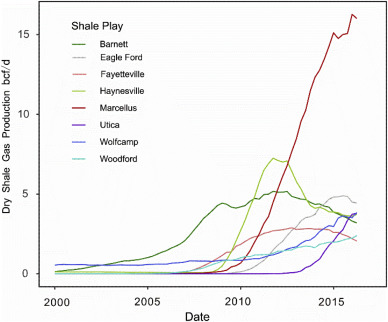
\includegraphics[height=0.5\textheight]{figures/example.jpg}
    \caption{Shale Gas Production per Area in each Well}
\end{figure}  
\end{column}
\begin{column}{0.5\textwidth}
\textbf{Causal Relations}
    \begin{itemize}
        \item Shale Gas Boom $\to$ Income
        \item Shale Gas Boom $\to$ Education
        \item HTE by Income Level
    \end{itemize}
\end{column}
\end{columns}

\begin{itemize}
    \item Rapid growth in natural resource industries generates numerous well-paying jobs that require relatively little formal education.
    \item As a result, young people may choose to work instead of staying in school leading to lower educational attainment
\end{itemize}
\end{frame}
%------------------------------------------------
% \begin{frame}{Distributional Effects: Dutch Blessing?}

% \textbf{Research Questions}

% \begin{itemize}
%     \item Did the Shale boom really undermine local educational attainment?
%     \item Was the effect uniform across different income groups?
% \end{itemize}

% \begin{figure}[htbp]
%   \centering
%   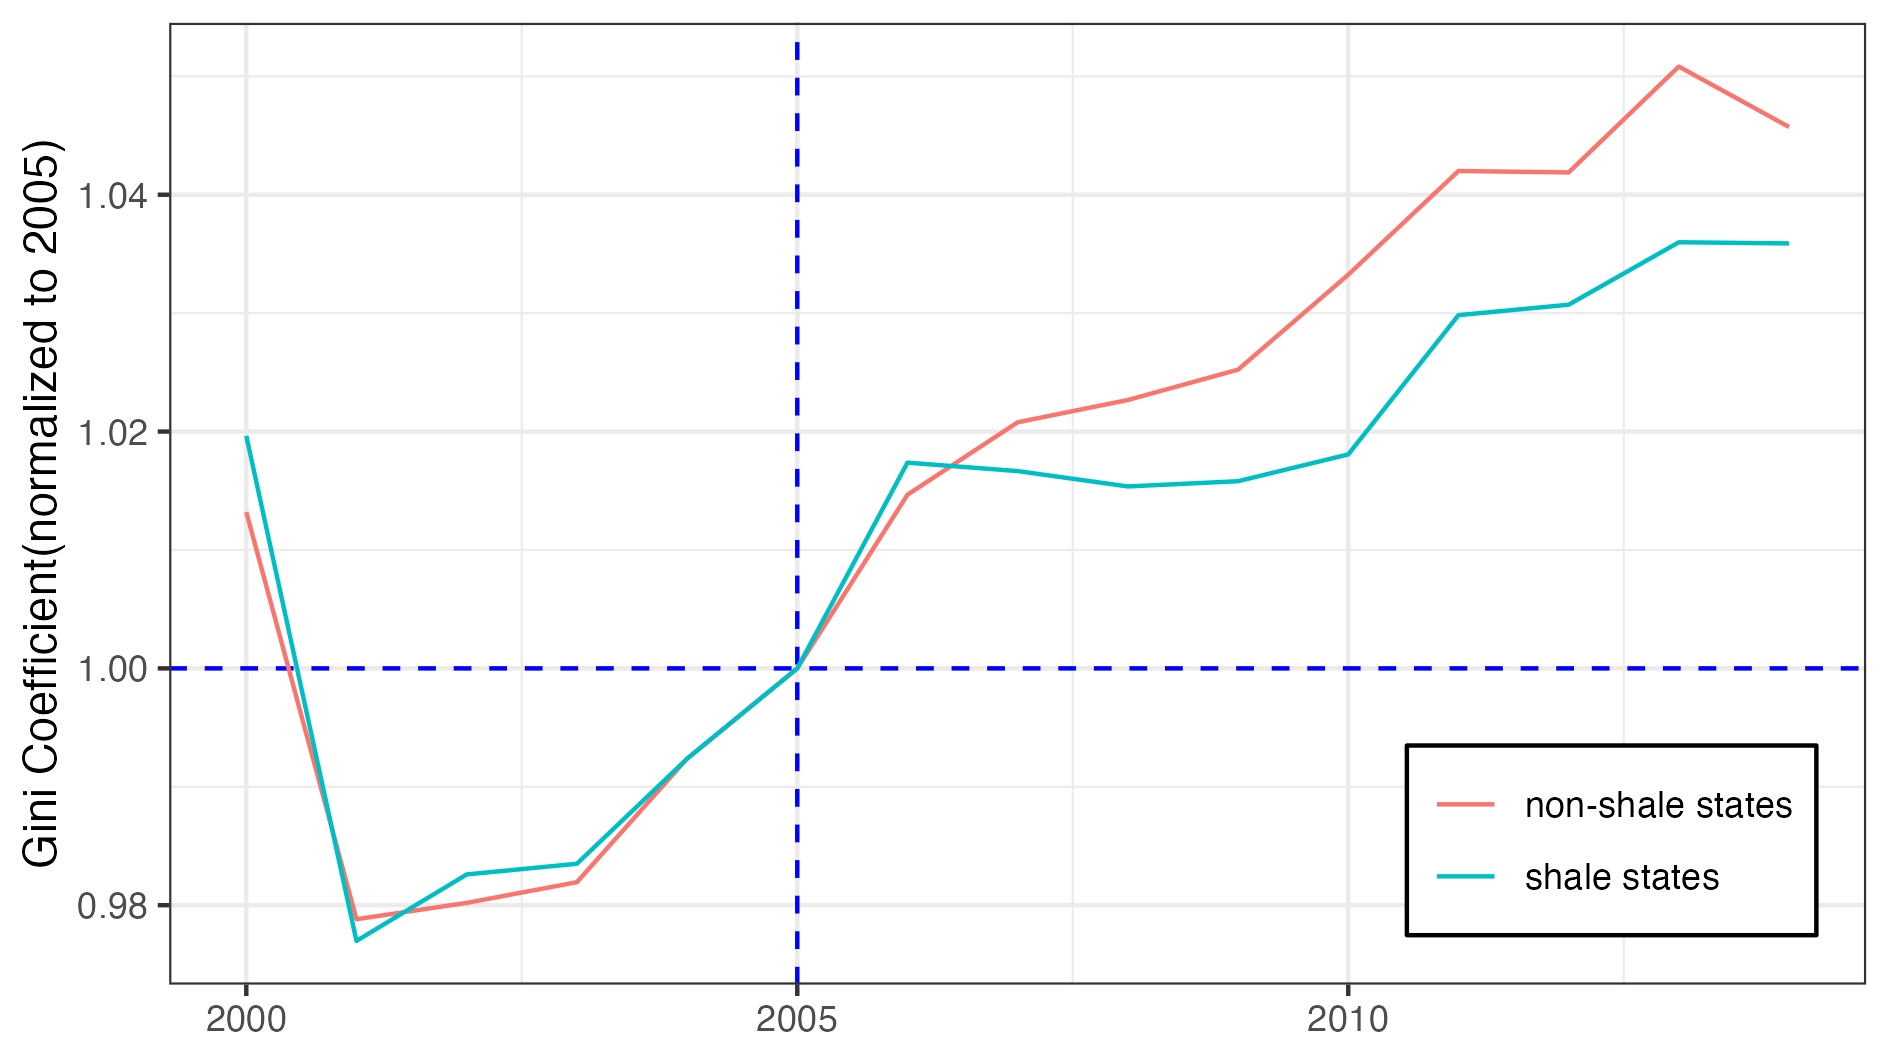
\includegraphics[width=0.6\textwidth]{figures/gini.png}
%   \caption{Gini Index Before and After the Shale Gas Shock}
%   \label{fig:gini}
% \end{figure}
% \end{frame}
%------------------------------------------------
% 2. Literature Review
\begin{frame}{Literature Review}
\begin{itemize}
    \item Positive Effects of Shale Gas Shock \textbf{on Income}
    \begin{itemize}
        \item \textcite{weinstein2011economic}
    \end{itemize}
    
    \item Negative Effects of Shale Gas Shock \textbf{on Education}
    \begin{itemize}
        \item \textcite{rickman2017shale}, \textcite{carpenter2019texas}
    \end{itemize}
\end{itemize}

\vspace{0.5cm}

\textbf{What these papers miss}

\begin{itemize}
        \item No discussions of \textbf{heterogeneous treatment effects}, especially by income level
        \begin{itemize}
            \item Resource booms might increase education for low-income households, but not for high-income households
        \end{itemize}
        \item They all focus on intra-state district-level comparisons, not cross-state comparisons
\end{itemize}
\end{frame}
%------------------------------------------------
\begin{frame}{IPUMS ACS Data}
    \footnotesize
    \begin{itemize}
        \item IPUMS ACS - 1yr from 2002 to 2010
        \item Variables of Interest: Household Income, \textbf{College Enrollment}, School Attendance, etc.
        \item Excluded five states: Hawaii, Alaska, Puerto Rico, Colorado, and Wyoming
    \end{itemize}
\begin{table}[ht]
\centering
\tiny
\begin{tabular}{l|l||c|c|ccc|ccc}
  \hline 
 & Age  & Observations & Weighted Population & \multicolumn{3}{c|}{Personal Income} & \multicolumn{3}{c}{Family Income} \\ 
 &  & & & Mean & Std. Dev. & Count & Mean & Std. Dev. & Count\\ 
  \hline 
   \multirow{4}{*}{Non-shale} & [5, 10] & 1,308,465.00 & 170,364,982.00 & NaN & -0.00 & 0.00 & 72,838.58 & 75,229.40 & 1,298,525.00 \\ 
   & [16, 18] & 716,276.00 & 89,493,317.00 & 2,152.02 & 5,346.15 & 716,139.00 & 76,209.93 & 75,288.26 & 684,920.00 \\ 
   & [18, 24] & 1,396,758.00 & 201,384,880.00 & 10,645.98 & 13,378.58 & 1,396,368.00 & 59,542.08 & 63,236.34 & 1,287,939.00 \\ 
   & total & 17,029,516.00 & 2,116,225,634.00 & 32,089.57 & 45,426.91 & 13,756,814.00 & 71,707.67 & 72,064.18 & 16,680,293.00 \\ 
   \multirow{4}{*}{Shale} & [5, 10] & 301,477.00 & 40,178,779.00 & NaN & -0.00 & 0.00 & 62,547.86 & 64,017.72 & 299,038.00 \\ 
   & [16, 18] & 162,607.00 & 20,788,610.00 & 2,107.18 & 5,266.69 & 162,587.00 & 67,489.58 & 66,903.25 & 155,650.00 \\ 
   & [18, 24] & 315,031.00 & 47,152,003.00 & 10,024.05 & 12,636.98 & 314,959.00 & 52,141.72 & 55,290.96 & 291,304.00 \\ 
   & total & 3,794,579.00 & 478,463,294.00 & 28,501.66 & 40,124.54 & 3,043,685.00 & 63,292.86 & 62,940.60 & 3,709,749.00 \\ 
   \hline \hline
   & Age & \multirow{10}{*}{} & \multirow{10}{*}{}& \multicolumn{3}{c|}{Education (Years)} & \multicolumn{3}{c}{College Enrollment} \\ 
  & &  & & Mean & Std. Dev. & Count  & Mean & Std. Dev. & Count  \\ 
  \hline
   \multirow{4}{*}{Non-shale} & [5, 10] & &  & 0.63 & 1.31 & 1,308,465.00 & 0.00 & 0.00 & 1,308,465.00 \\ 
   & [16, 18] & &  & 10.60 & 1.32 & 716,276.00 & 0.23 & 0.42 & 716,276.00 \\ 
   & [18, 24] &  &  & 12.37 & 2.02 & 1,396,758.00 & 0.82 & 0.39 & 1,396,758.00 \\ 
   & total &  & & 11.14 & 5.28 & 16,429,863.00 & 0.64 & 0.48 & 17,029,516.00 \\ 
   \multirow{4}{*}{Shale}& [5, 10] &  &  & 0.60 & 1.25 & 301,477.00 & 0.00 & 0.00 & 301,477.00 \\ 
   & [16, 18] &  &  & 10.48 & 1.40 & 162,607.00 & 0.21 & 0.41 & 162,607.00 \\ 
   & [18, 24] &  &  & 12.22 & 2.00 & 315,031.00 & 0.80 & 0.40 & 315,031.00 \\ 
   & total &  &  & 10.74 & 5.21 & 3,656,064.00 & 0.61 & 0.49 & 3,794,579.00 \\ 
   \hline
\end{tabular}
\caption{Summary Statistics} 
\label{tab:sum_stat}
\end{table}

\end{frame}
%------------------------------------------------
\begin{frame}{Methodology: \textcite{sun_estimating_2021} DiD}

In our case of shale gas boom, the treatment assignment is staggered across states.
    \begin{columns}
    \column{0.47\linewidth}
\begin{table}[htbp]
    \centering
    \begin{tabular}{c| c}
        
        Year & State \\
        \hline \hline
        2005 & Texas \\
        2006 & Arkansas \\
        2006 & Oklahoma \\
        2008 & Alabama \\
        2008 & Louisiana \\
        2008 & Pennsylvania \\
        2008 & West Virginia \\
    \end{tabular}
    \caption{Shale Gas Extraction Beginnings by State}
    \label{tab:shale-gas-extraction}
\end{table}
    \column{0.06\linewidth}
    \centering
    \Huge
    =
    \column{0.47\linewidth}
    \begin{table}[h]
        \centering
        \begin{tabular}{|c|c|c|c|c|c|}
        \hline
             &$t_1$&$t_2$&$t_3$&$t_4$&$t_5$  \\ \hline
             $g_1$&\textcolor{red!60}{o}&\textcolor{red!60}{o}&\textcolor{red!60}{o}&\textcolor{red!60}{o}&\textcolor{red!60}{o}  \\ \hline
             $g_2$&x&\textcolor{red!60}{o}&\textcolor{red!60}{o}&\textcolor{red!60}{o}&\textcolor{red!60}{o}  \\ \hline
             $g_3$&x&x&\textcolor{red!60}{o}&\textcolor{red!60}{o}&\textcolor{red!60}{o} \\ \hline
             $g_4$&x&x&x&\textcolor{red!60}{o}&\textcolor{red!60}{o}  \\ \hline
             $g_5$&x&x&x&x&\textcolor{red!60}{o}  \\ \hline
             $g_\infty$&x&x&x&x&x  \\ \hline
        \end{tabular}
        \caption{Staggered Adoption}
        % \label{tab:my_label}
    \end{table}
\end{columns}

\end{frame}
%------------------------------------------------
\begin{frame}{Assumptions for Causal identification}
\begin{wideitemize}
    \item \textcite{sun_estimating_2021} DiD
    \begin{itemize}
        \item \textbf{Parallel Trends}: The treated and control groups would have followed the same trend in the absence of treatment
        \item \textbf{No Compositional Changes}: The composition of the treated and control groups remains constant over time
        \item \textbf{Homogeneity of Dynamic Treatment Effects}: The dynamic evolution of treatment effect is the same across different shale states
    \end{itemize}
\end{wideitemize}
\end{frame}
%------------------------------------------------
\begin{frame}{Main Result: Income}
\vfill
    \begin{itemize}
        \item Household income increased by 2.5\% overall in the third year after the shale boom.
        \item In 1Q, the increase was 18\%; in 2Q, it was 5\%; in 3-4Q, it was not statistically significant.
    \end{itemize}
\begin{figure}[htbp]
    \centering
    \begin{minipage}{0.45\textwidth}
        \centering
        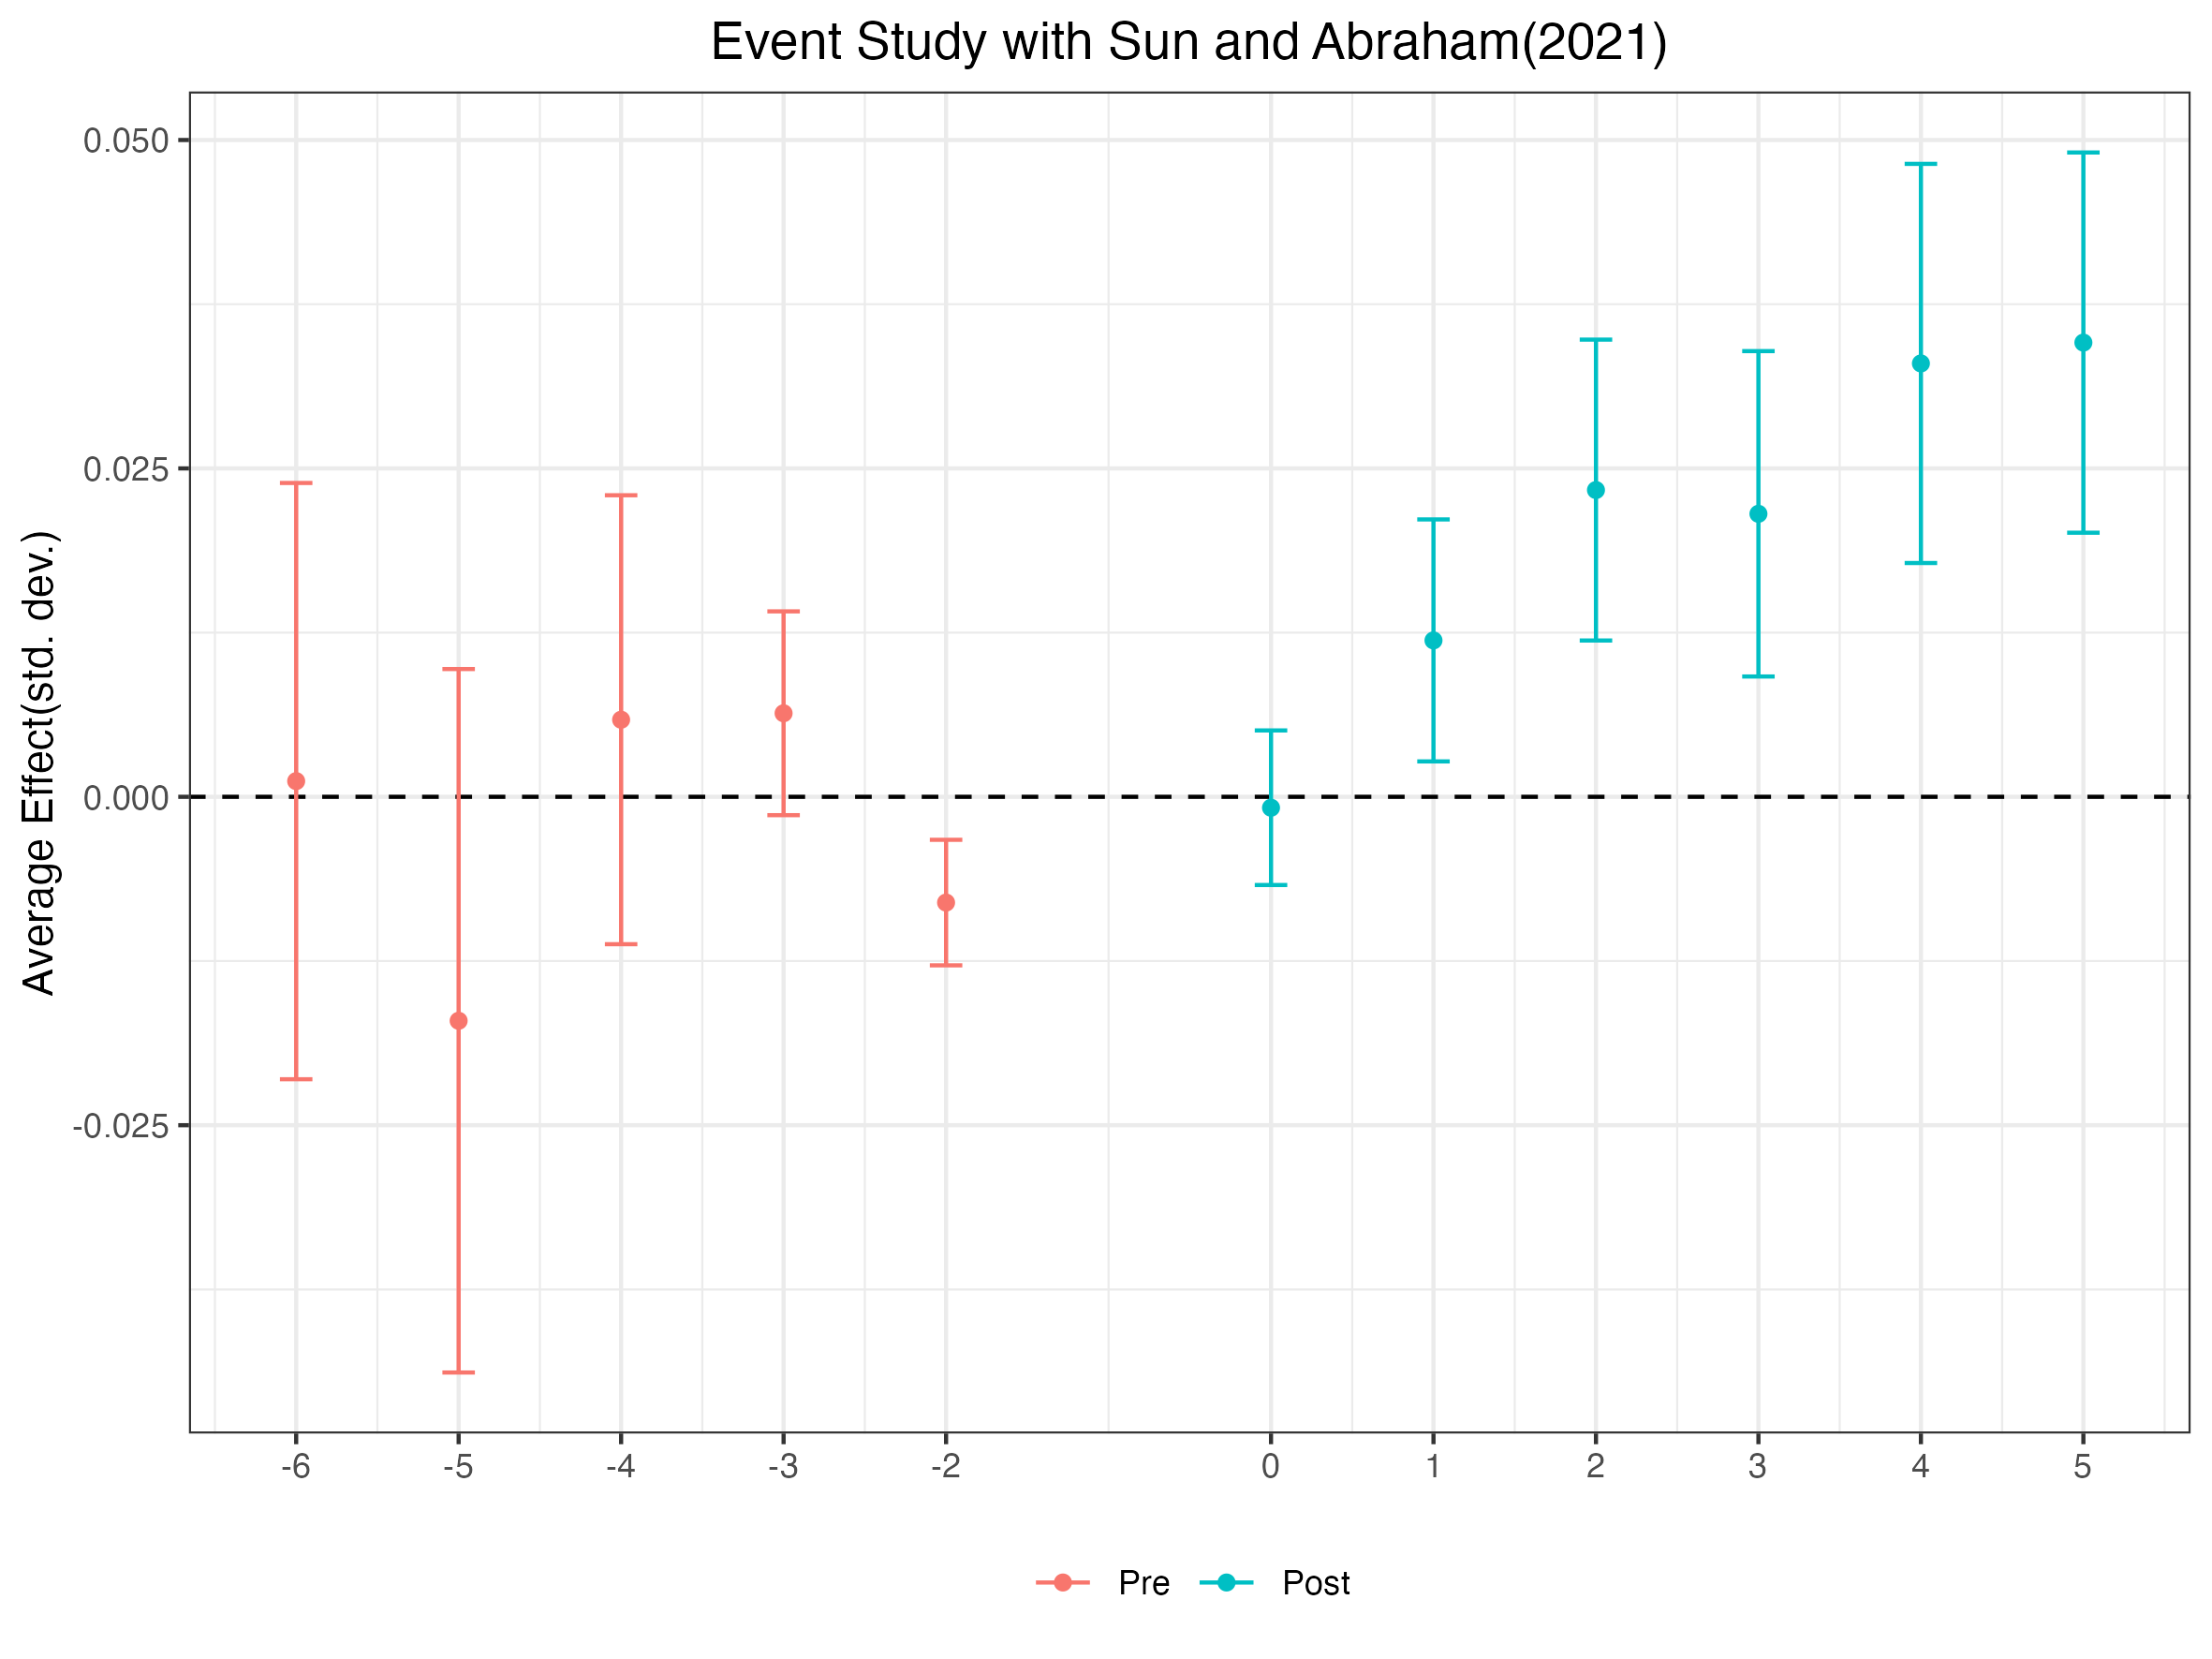
\includegraphics[width=\linewidth, height=4cm]{figures/did-base/sadid(logFTOTINC).png}
        \caption{Overall Income}
        \label{fig:Overall Income}
    \end{minipage}
 \hfill
    \begin{minipage}{0.45\textwidth}
    \centering
    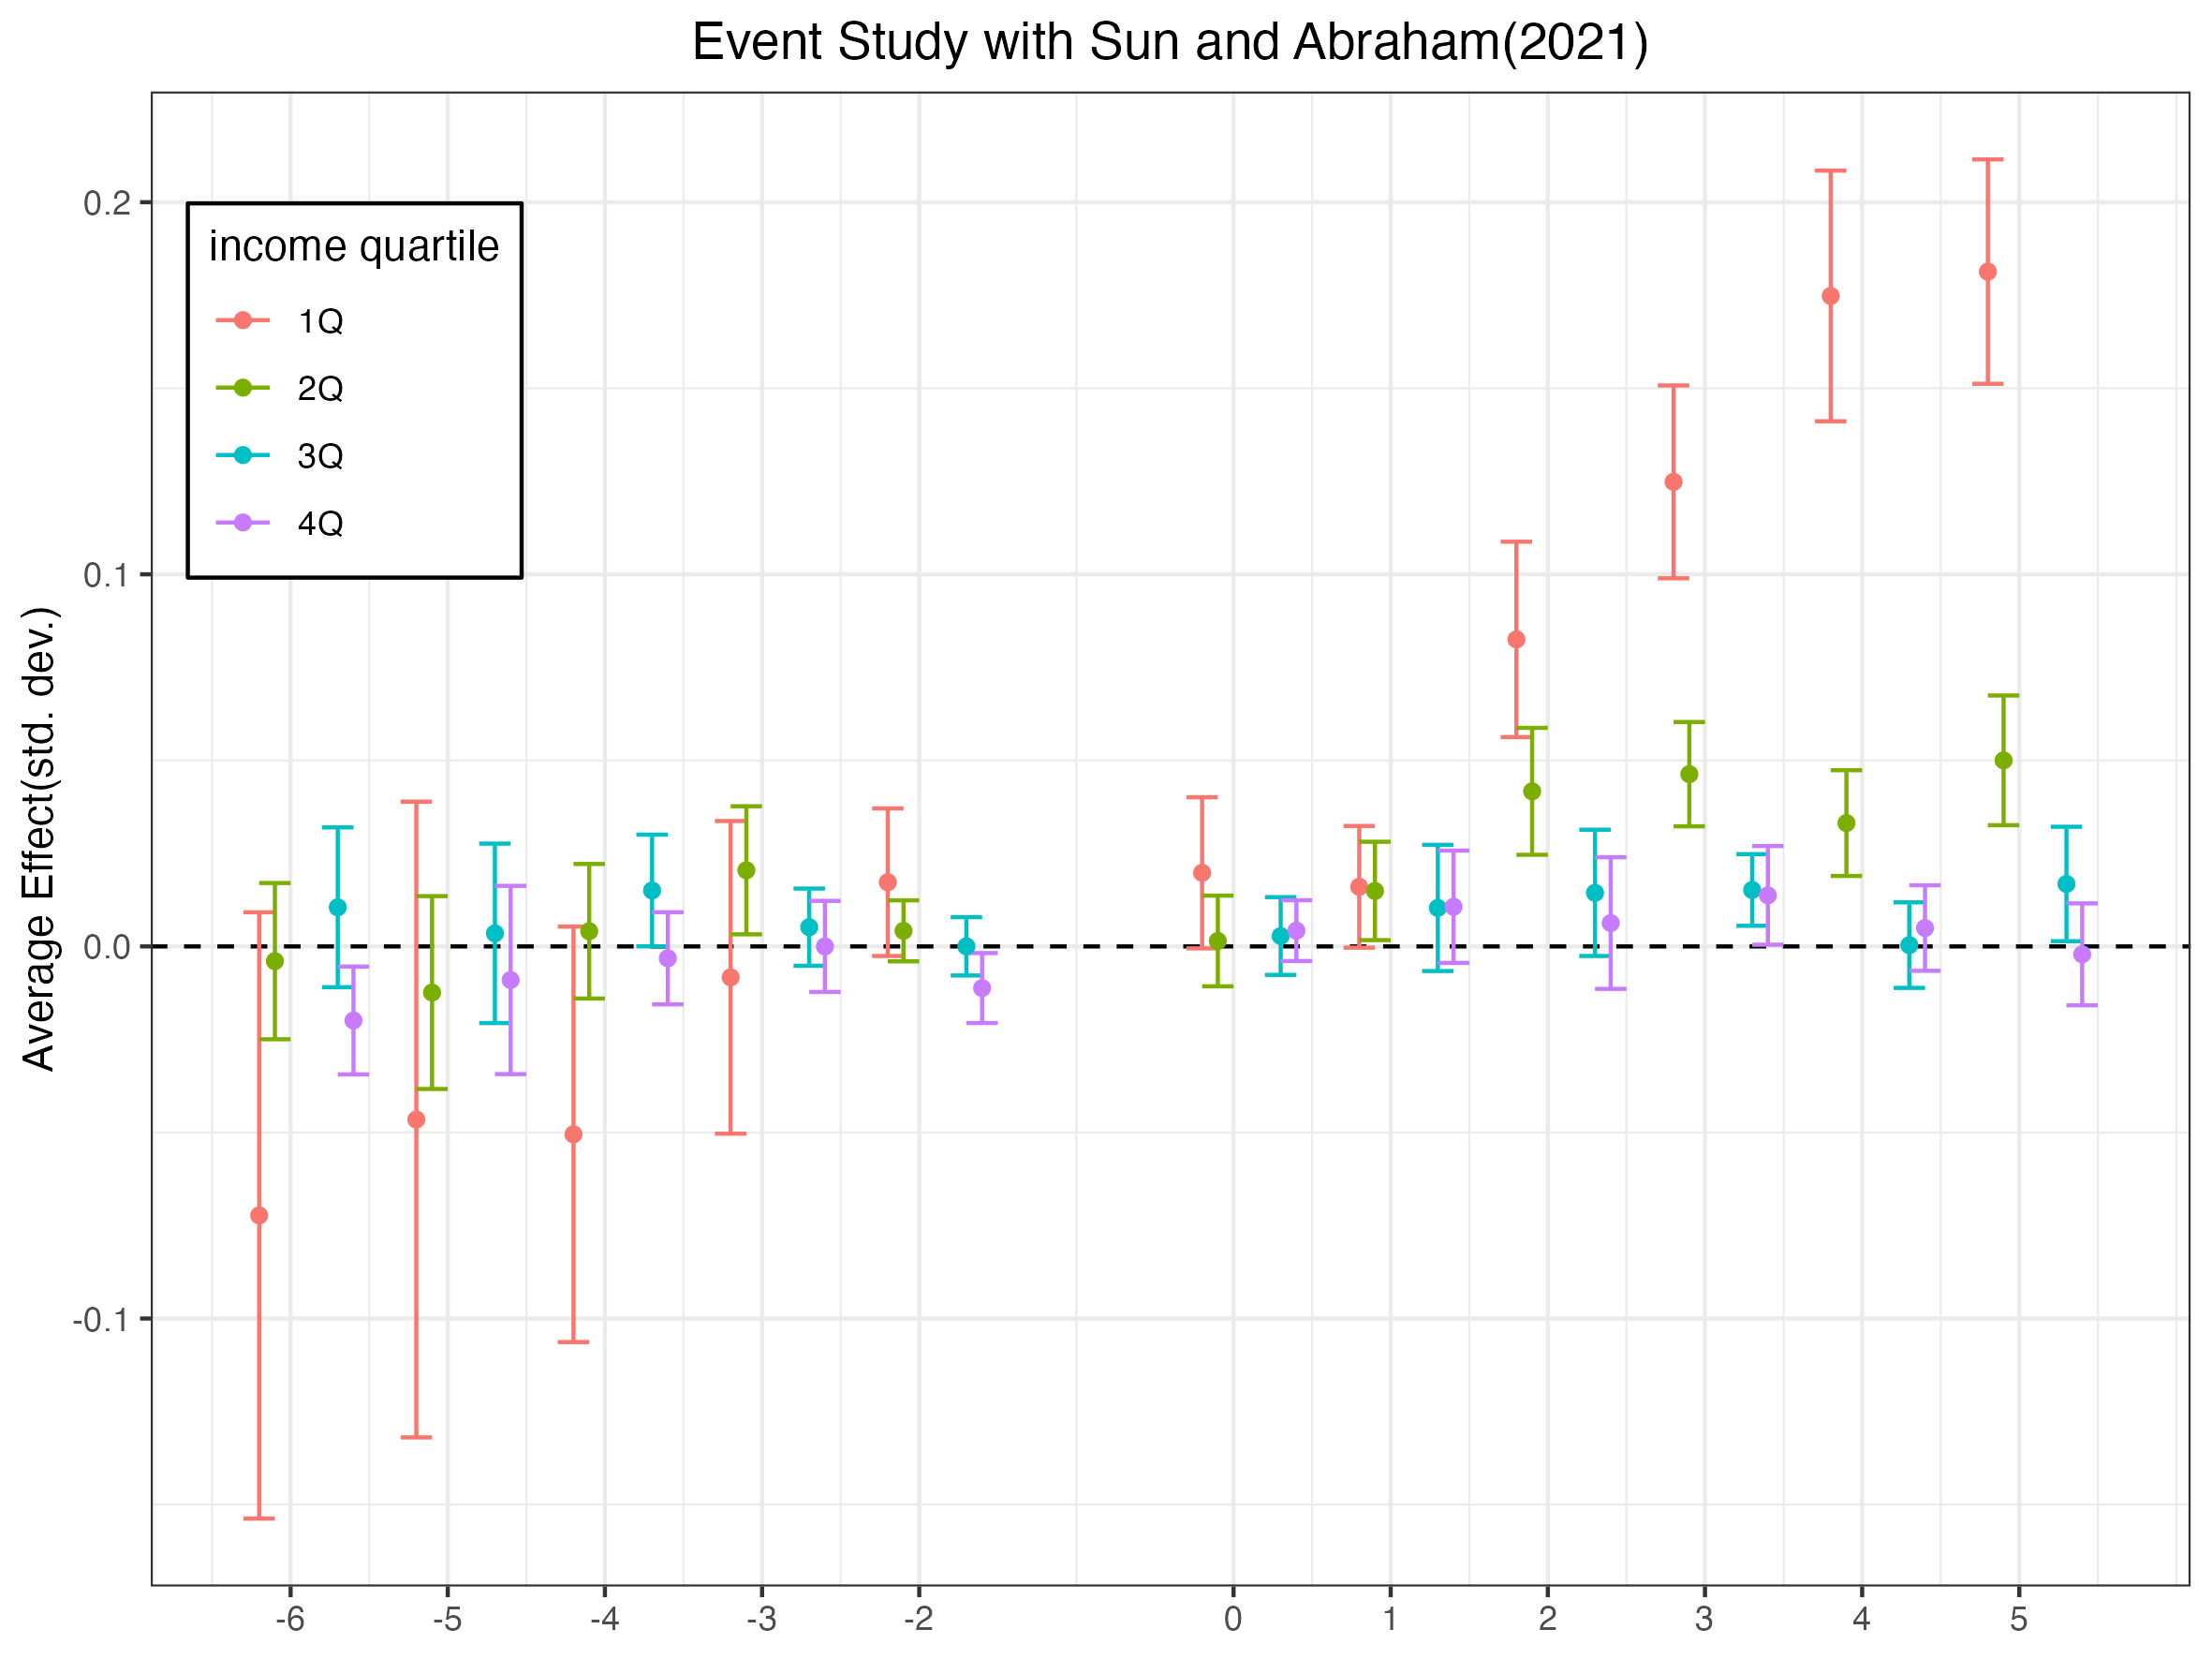
\includegraphics[width=\linewidth, height=4cm]{figures/did-base/sadid(logINCTOT - by income quartile).png}
    \caption{Income by Quartile}
    \label{fig:Income by Quartile}
    \end{minipage}
\end{figure}
\end{frame}
%------------------------------------------------
\begin{frame}{Main Result: Education}
    \vfill
    \begin{itemize}
        \item College enrollment increased by 7.5\%p overall in the third year after the shale boom.
        \item The increase was mainly driven by the 1Q households.
        \item Drawback: Violation in the parallel trend assumptions in the left figure
    \end{itemize}
\begin{figure}[htbp]
    \centering
    \begin{minipage}{0.45\textwidth}
        \centering
        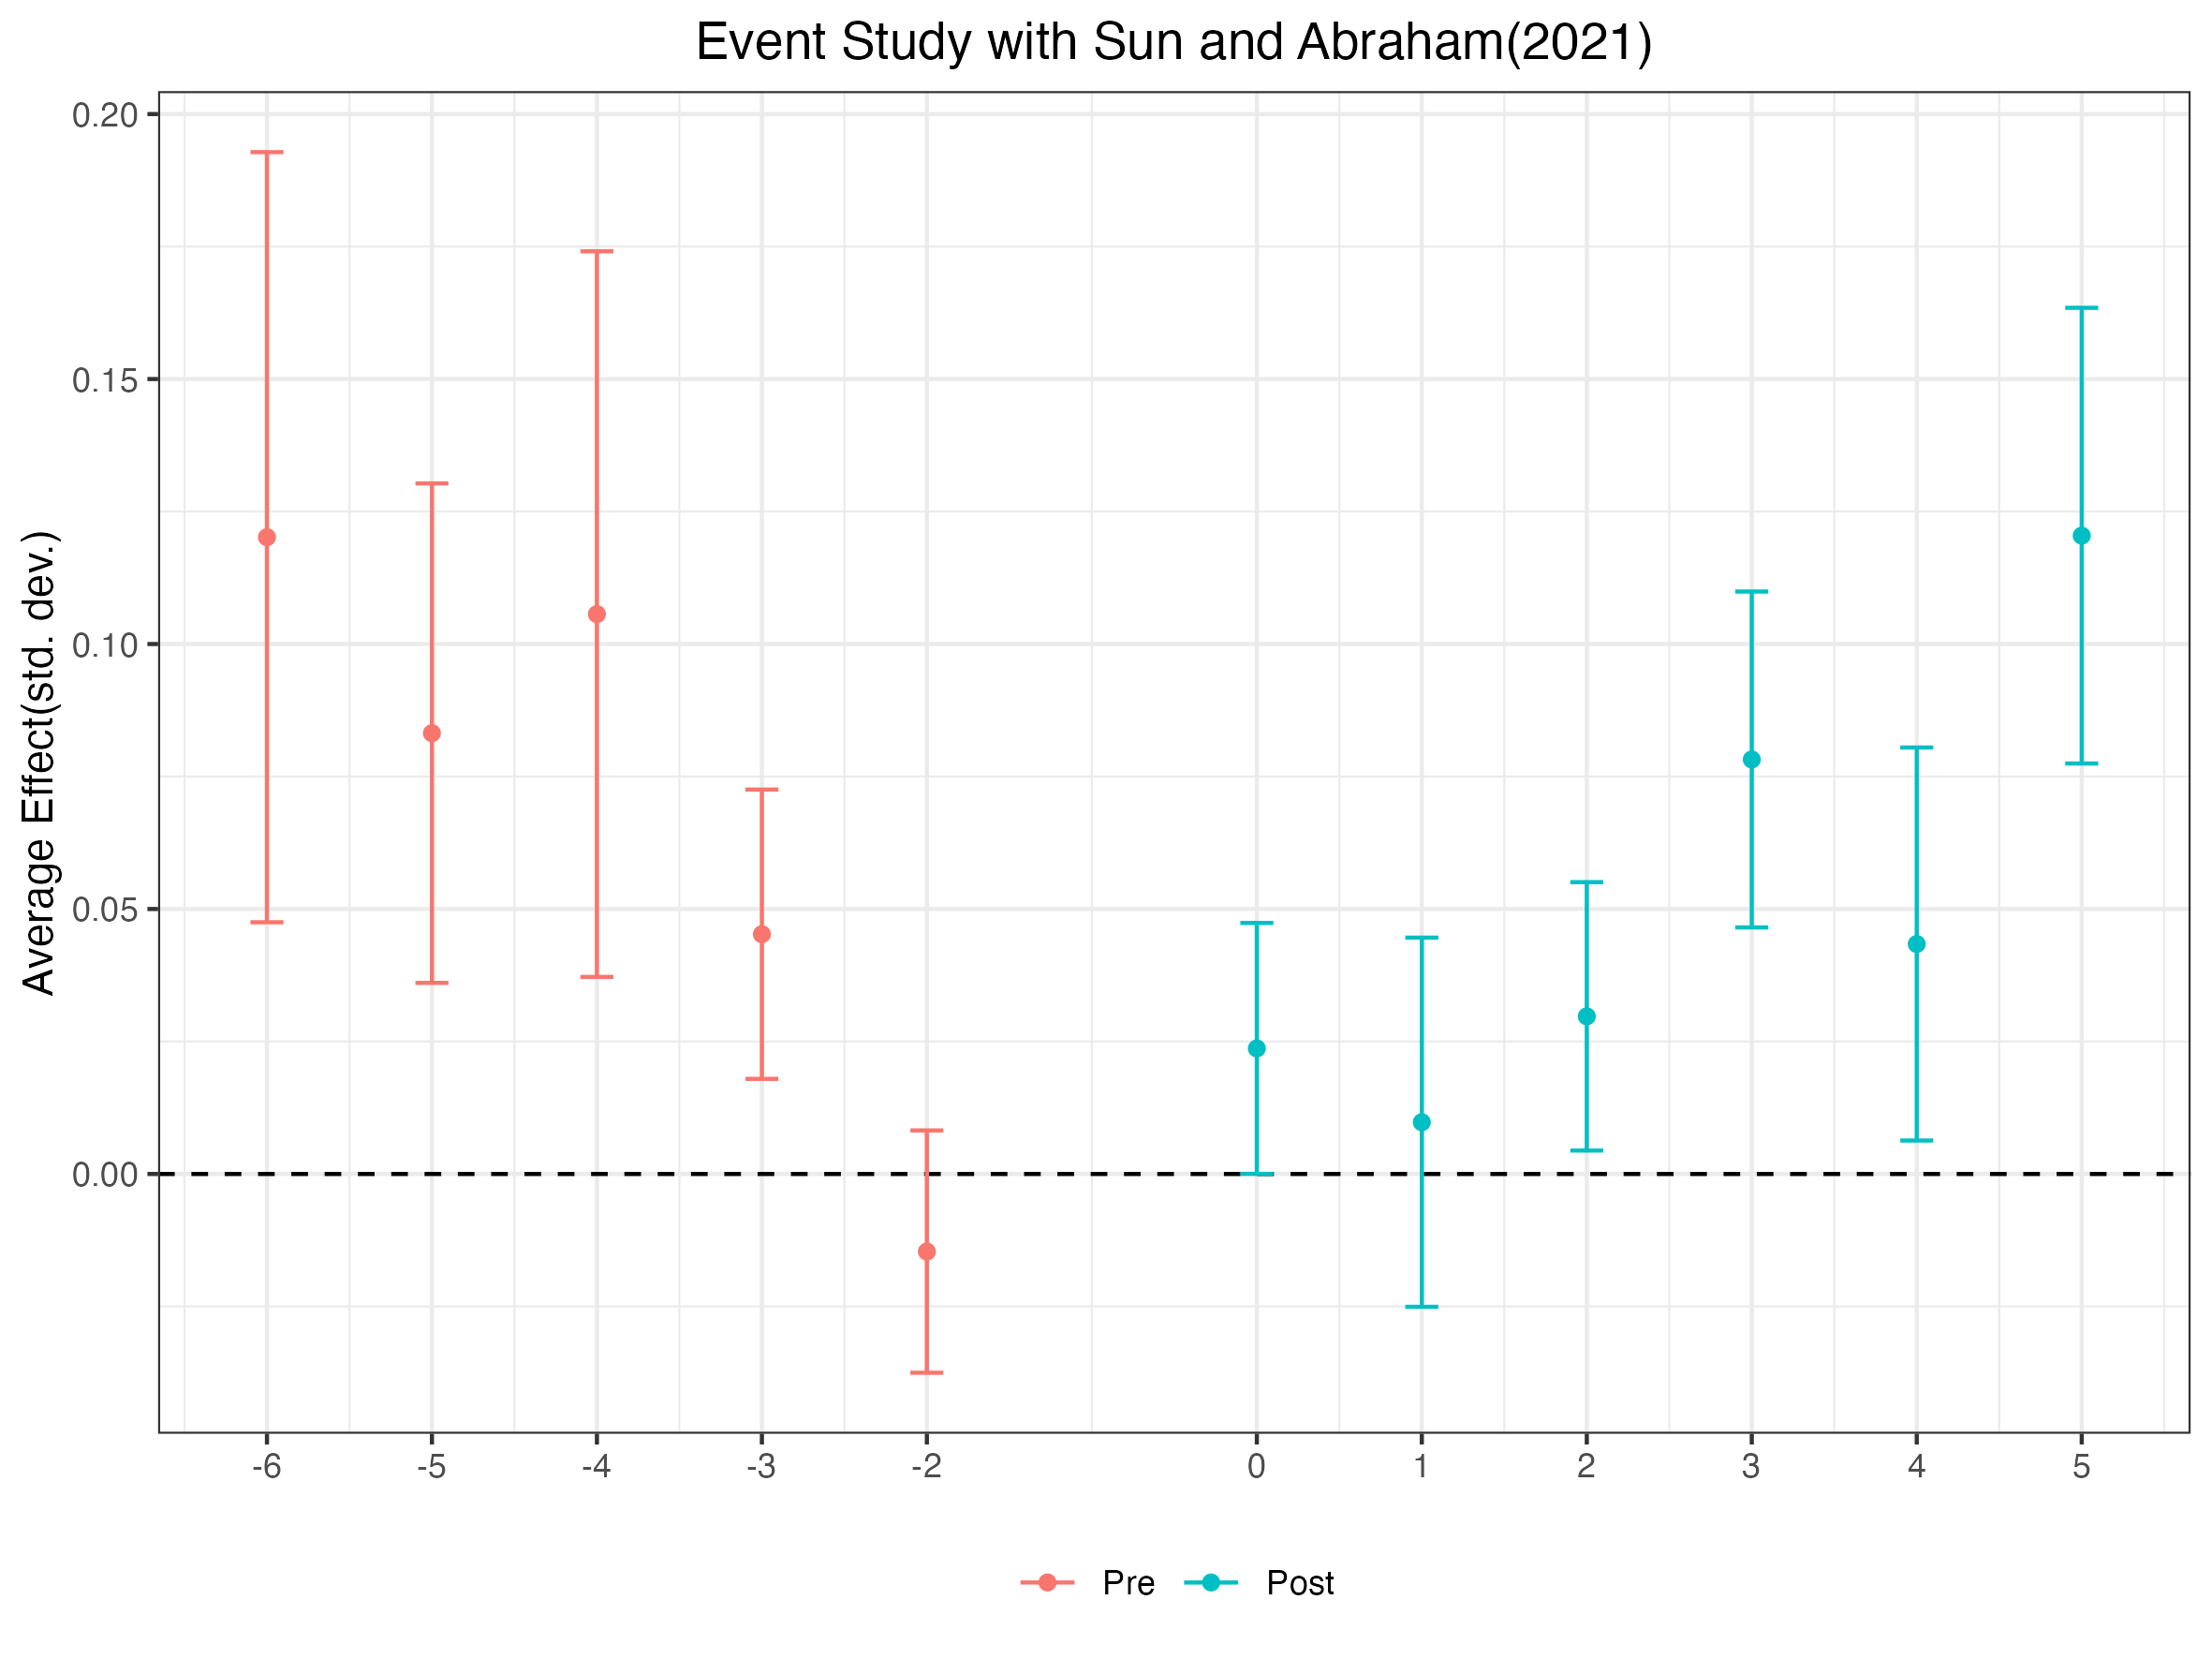
\includegraphics[width=\linewidth]{figures/did-base/sadid(college enrollment).png}
        \caption{College Enrollment}
        \label{fig:college enrollment}
    \end{minipage}
    \hfill
    \begin{minipage}{0.45\textwidth}
        \centering
        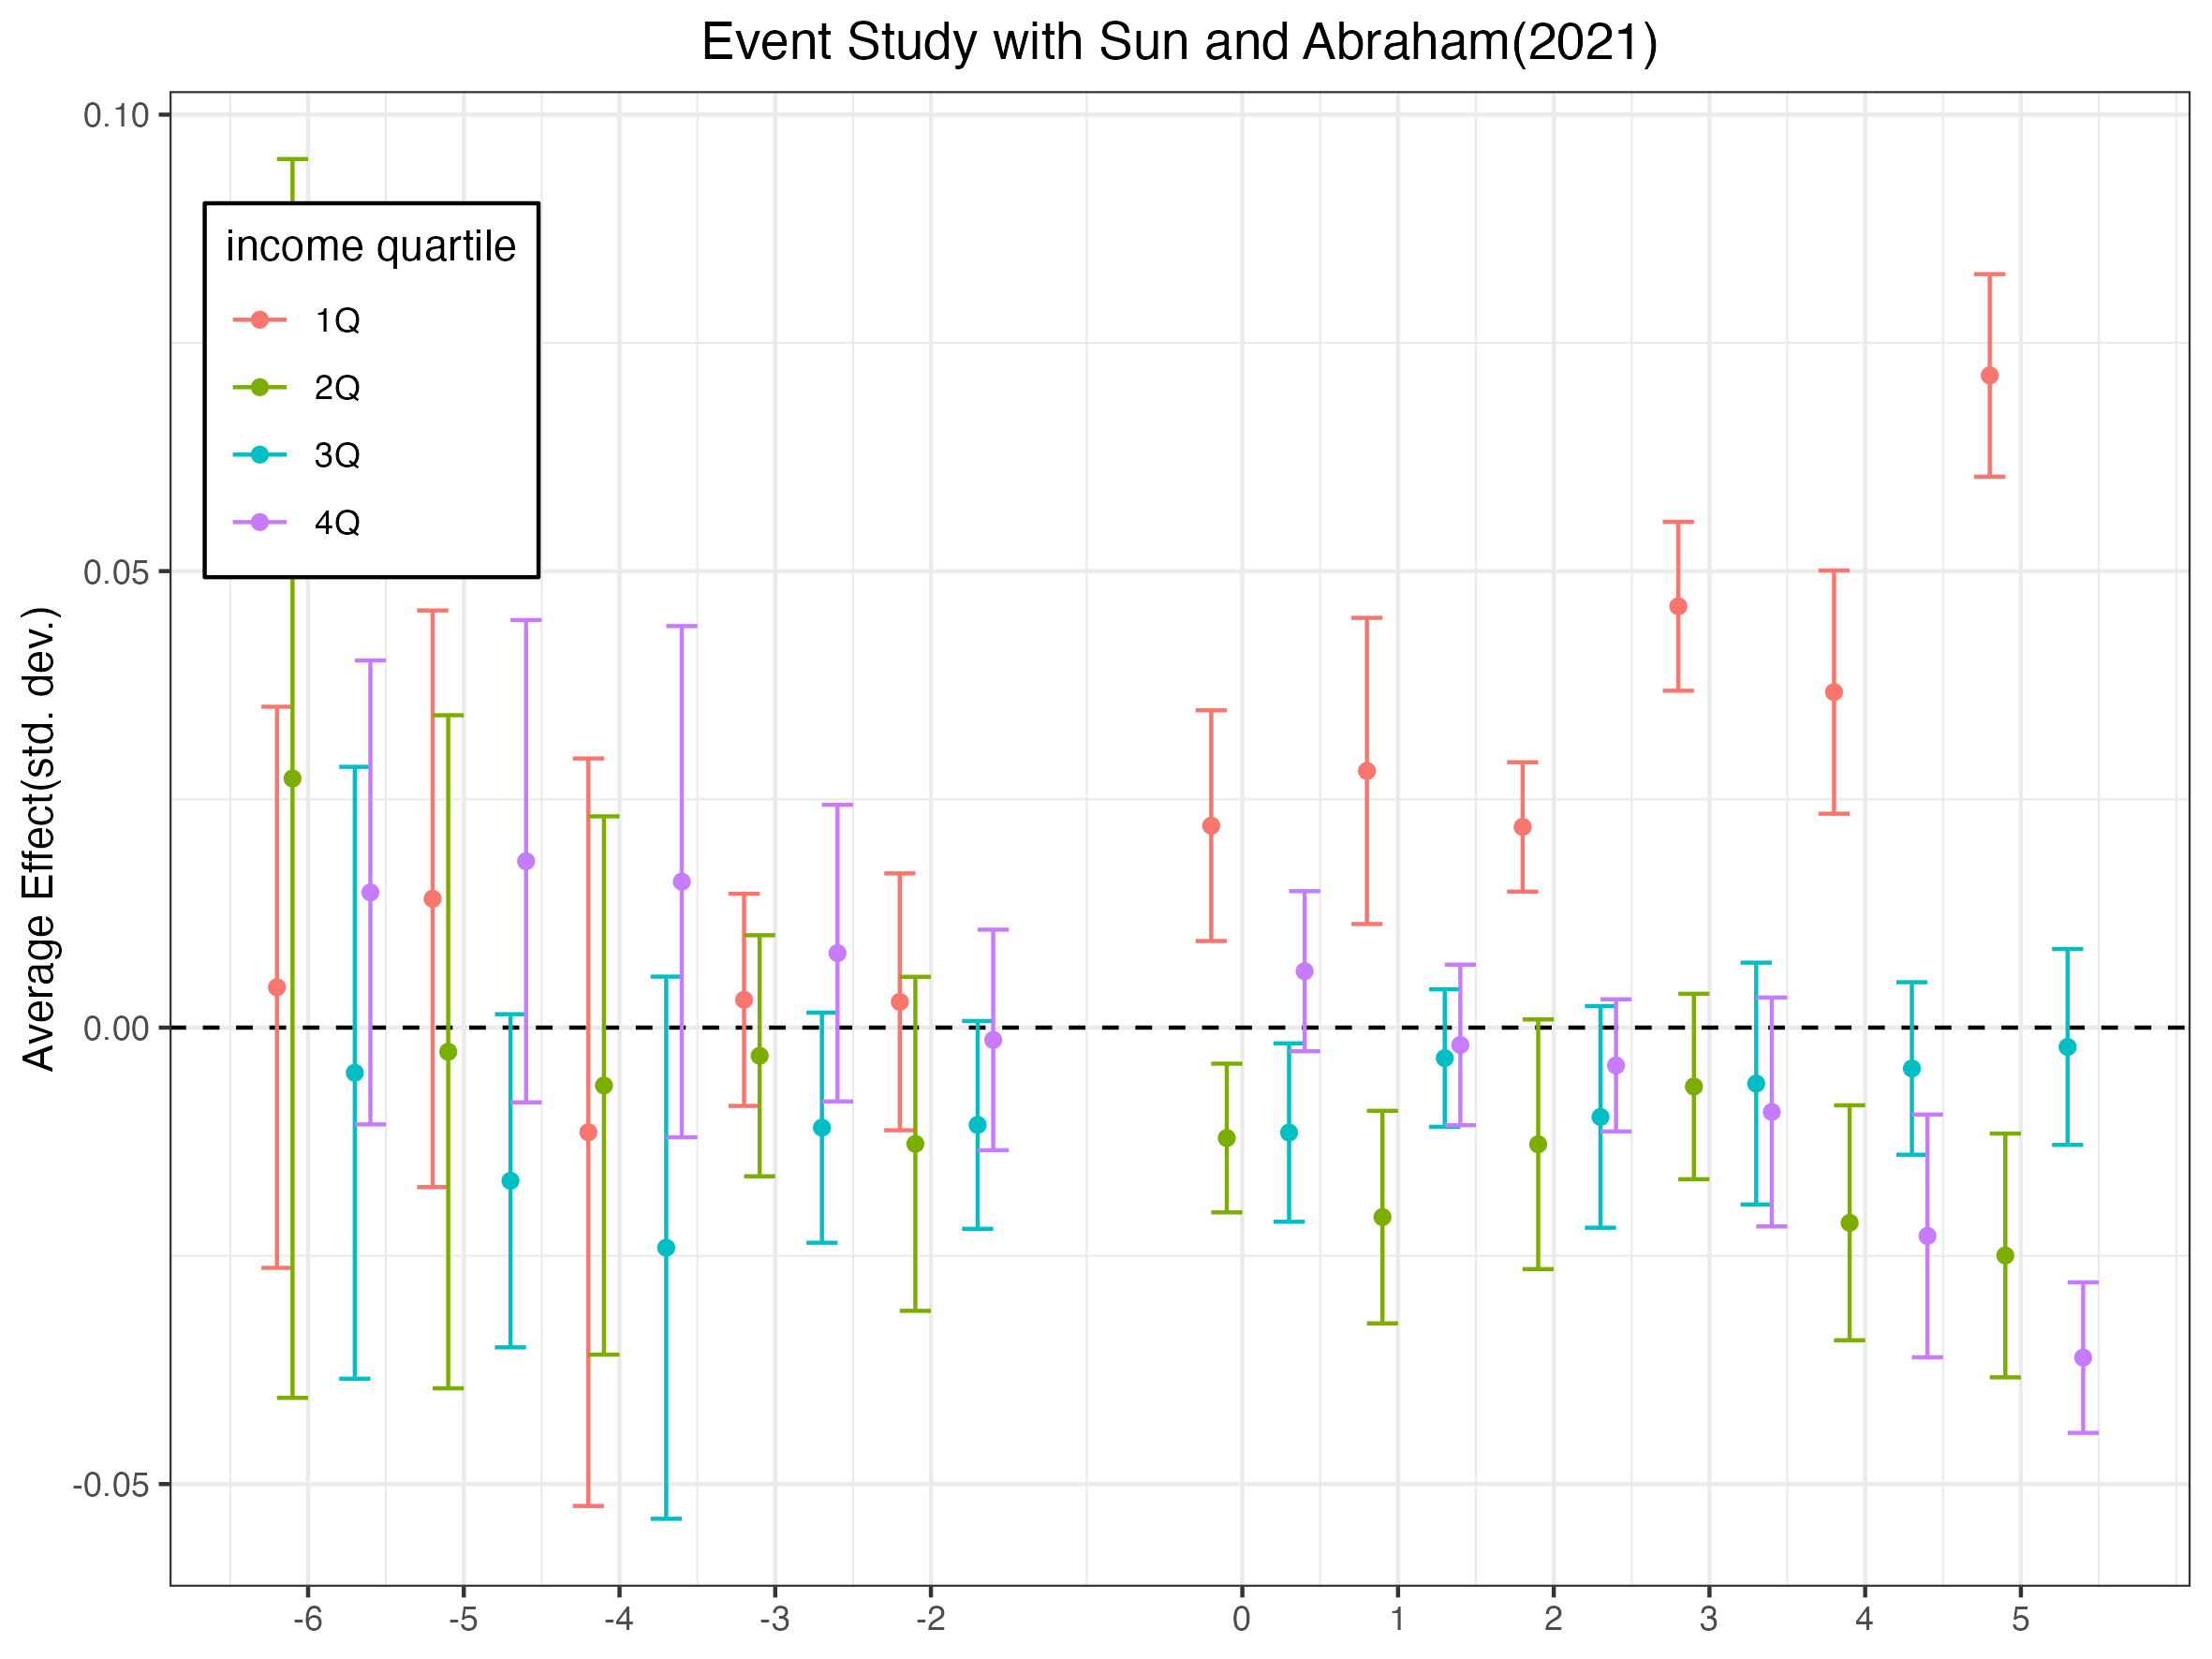
\includegraphics[width=\linewidth]{figures/did-base/sadid(college share - by income quartile).png}
        \caption{College Share by Income Quartile}
        \label{fig:college shares}
    \end{minipage}
\end{figure}
\end{frame}


%------------------------------------------------
% \begin{frame}{Conclusion}
% \begin{wideitemize}
%     \item Shale gas boom increased income and college enrollment especially for low-income households
%     \item Our analysis challenge conventional “Dutch Disease” rather suggesting a “Dutch Blessing” of resource-driven shock
%     \item Limitations
%     \begin{itemize}
%         \item Focused on short- to medium-run effects
%         \item Did not capture spillovers across states 
%         % \item Possible bias from unobserved confounders might still persist
%     \end{itemize}  
% \end{wideitemize}
% \end{frame}
%------------------------------------------------
\begin{frame}{Future Work}

\begin{wideitemize}
    \item What kind of microdata can I add to this research?
    \item How can I incorporate ML methods such as causal forest to this research?
    \begin{wideitemize}
        \item \textcite{wang2024longbet} proposes the following method to estimate CATT in panel data settings:
        \item Assumptions: Unconfoundedness, Overlap
        \item Outcome Model 
        \begin{align*}
            Y_{it} = \alpha \mu(X_i, T = t) + \beta_S \nu(X_i, S_{it},T = t) + \epsilon_{it}
        \end{align*}
        where $S$ is the length to exposure (Train XBART forests separately for $\mu$ and $\nu$)
        \item CATT: \begin{align*}
            \tau_t(X_i, S) &\equiv  \mathbb{E}[Y_{it} | X_i, S_{it} = S] - \mathbb{E}[Y_{it} | X_i, S_{it} = 0] \\
            &= \beta_S \nu(X_i, S_{it}, T = t) - \beta_0 \nu(X_i, S=0, T = t)
        \end{align*}
    \end{wideitemize}
\end{wideitemize}

\end{frame}
%------------------------------------------------

\begin{frame}{References}
\tiny
\printbibliography[heading=none]
\end{frame}
%------------------------------------------------
\begin{frame}{Extensions: Other Educational Outcomes}
\begin{figure}[htbp]
    \centering
    \begin{minipage}{0.48\textwidth}
        \centering
        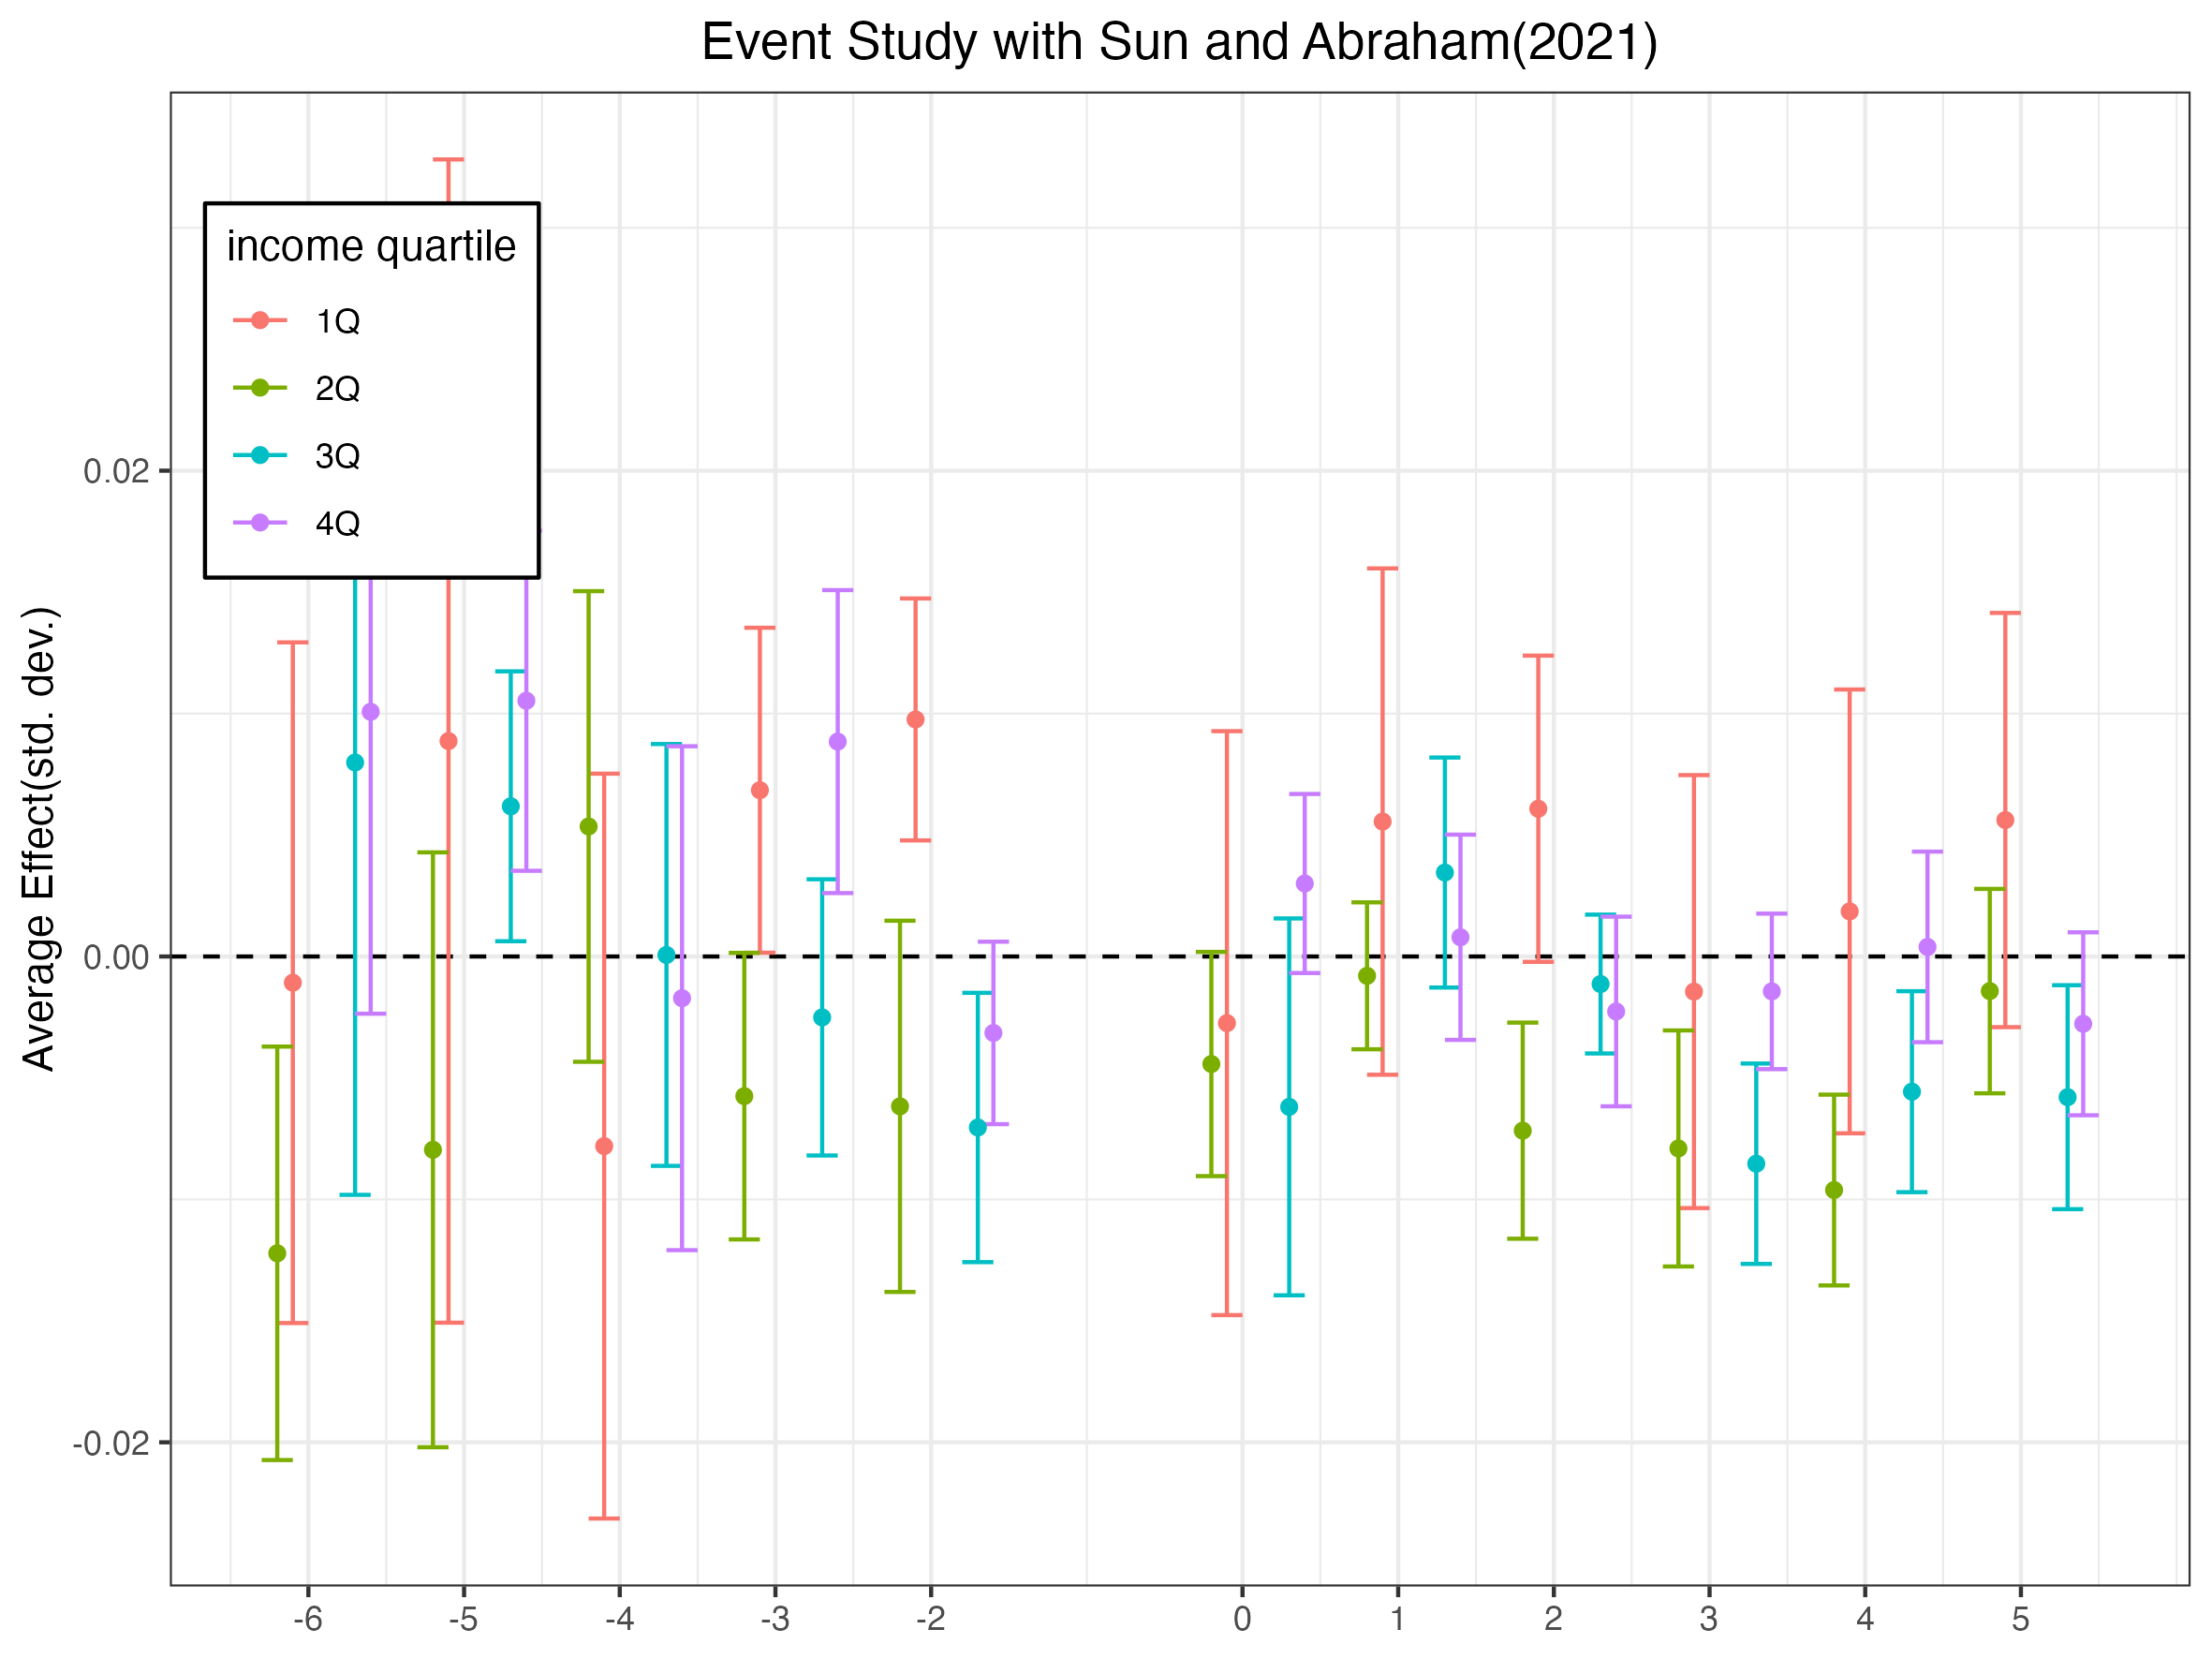
\includegraphics[width=\linewidth]{figures/did-base/sadid(young school attendance - by income quartile).png}
        \caption{Elementary School Attendance by Income Quartile}
        \label{fig:young school attendance by income quartile}
    \end{minipage}%
    \hfill
    \begin{minipage}{0.48\textwidth}
        \centering
        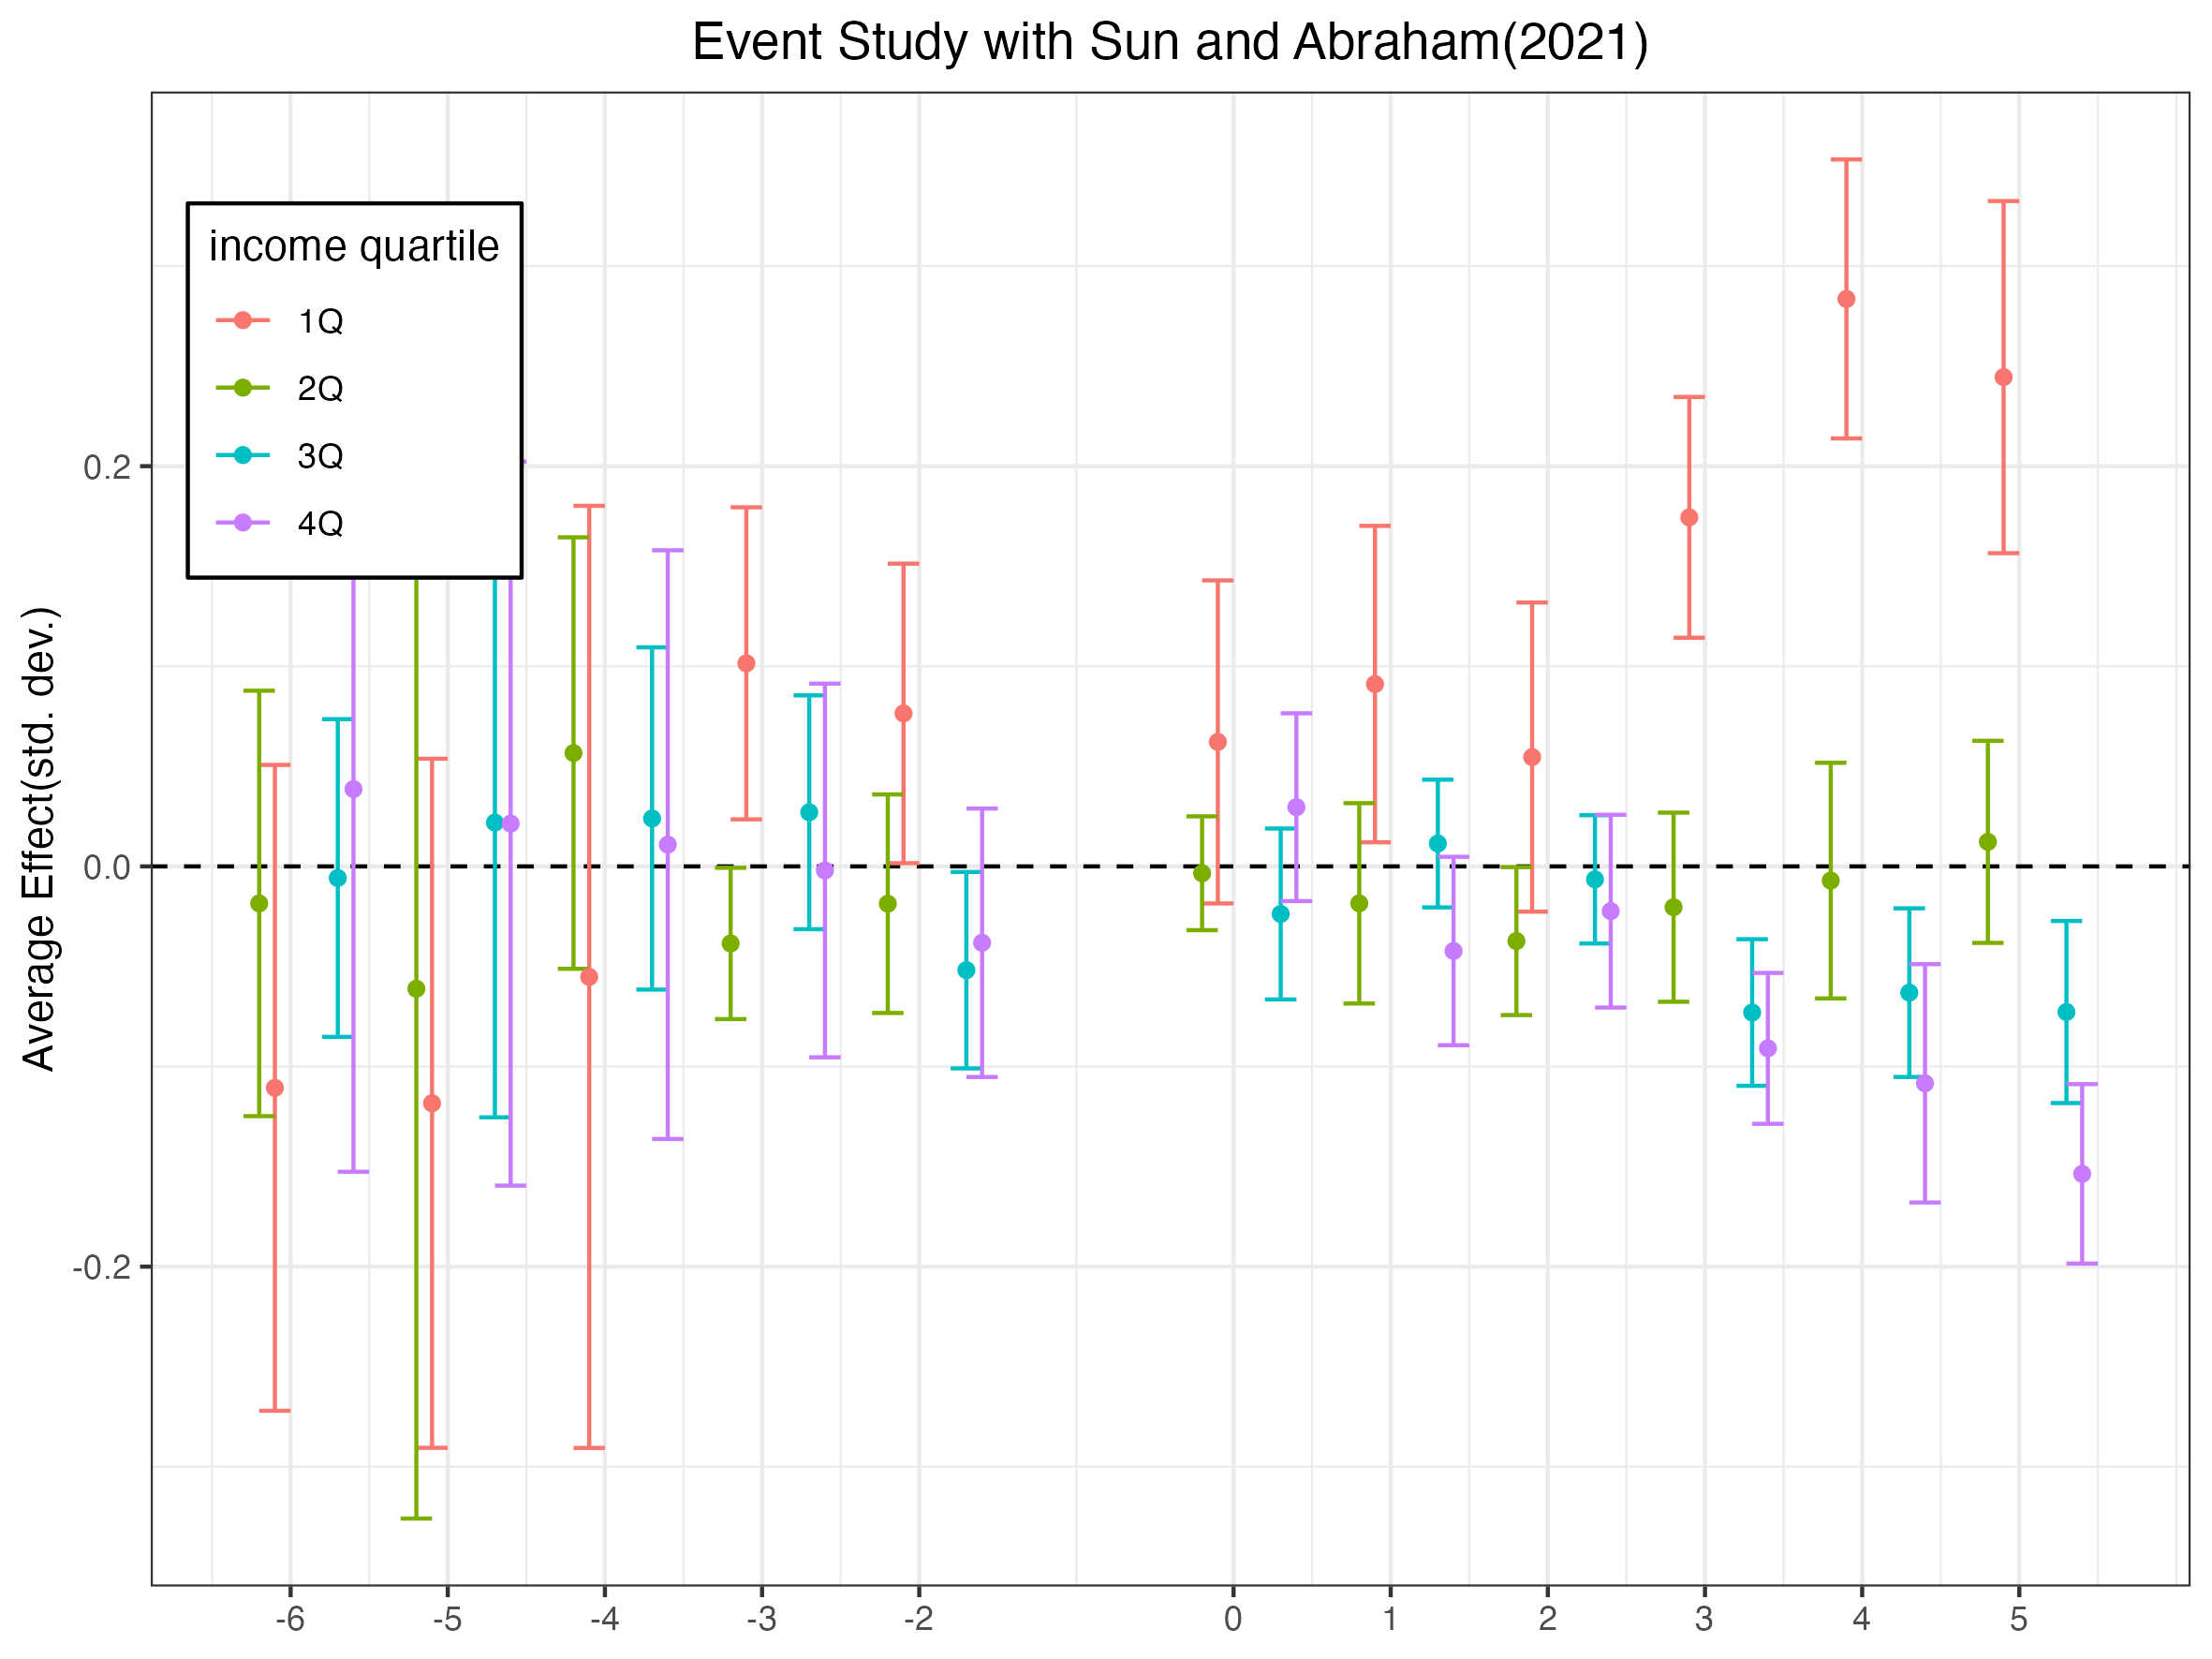
\includegraphics[width=\linewidth]{figures/did-base/sadid(high school attendance- by income quartile).png}
        \caption{High School Attendance by Income Quartile}
        \label{fig:high school attendance by income quartile}
    \end{minipage}
\end{figure}
\end{frame}


\end{document}
